\documentclass[12pt, letterpaper]{article}
\usepackage{amsmath}
\usepackage{amssymb}
\usepackage{tikz}
\usepackage[utf8]{inputenc}
\usetikzlibrary{patterns,arrows,decorations.pathreplacing}
\usepackage{xcolor}
\usetikzlibrary{patterns}

\begin{document}

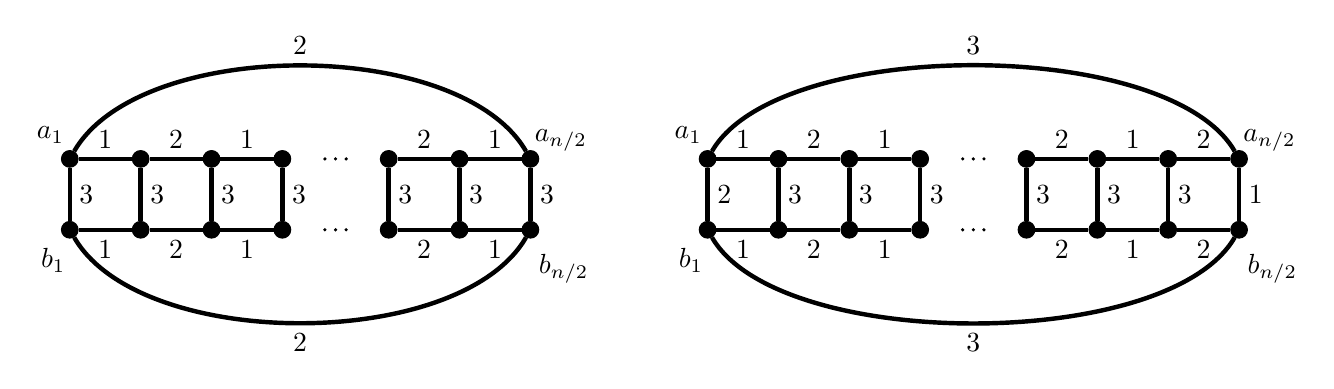
\begin{tikzpicture}[scale=0.9]
  \tikzstyle{vertex}=[draw,circle,fill=black,minimum size=6,inner sep=0]
  
  \node[vertex] (a1) at (1,1) [label={[xshift=-7pt, yshift=-1pt] $a_1$}] {};
  \node[vertex] (a2) at (2,1) {};
  \node[vertex] (a3) at (3,1) {};
  \node[vertex] (a4) at (4,1) {};
  \node[vertex] (a5) at (5.5,1) {};
  \node[vertex] (a6) at (6.5,1) {};
  \node[vertex] (a7) at (7.5,1) [label={[xshift=11pt, yshift=-4pt] $a_{n/2}$}] {};
  \node[vertex] (b1) at (1,0) [label={[xshift=-6pt, yshift=-22pt] $b_1$}] {};
  \node[vertex] (b2) at (2,0) {};
  \node[vertex] (b3) at (3,0) {};
  \node[vertex] (b4) at (4,0) {};
  \node[vertex] (b5) at (5.5,0) {};
  \node[vertex] (b6) at (6.5,0) {};
  \node[vertex] (b7) at (7.5,0) [label={[xshift=12pt, yshift=-26pt] $b_{n/2}$}] {};
  
  \draw[fill] (4.6,1) circle (0.4pt);
  \draw[fill] (4.75,1) circle (0.4pt);
  \draw[fill] (4.9,1) circle (0.4pt);
  
  \draw[fill] (4.6,0) circle (0.4pt);
  \draw[fill] (4.75,0) circle (0.4pt);
  \draw[fill] (4.9,0) circle (0.4pt);
  
  \draw[ultra thick] (a1) -- (a2) node[midway, yshift=7pt] {1};
  \draw[ultra thick] (a2) -- (a3) node[midway, yshift=7pt] {2};
  \draw[ultra thick] (a3) -- (a4) node[midway, yshift=7pt] {1};
  \draw[ultra thick] (a5) -- (a6) node[midway, yshift=7pt] {2};
  \draw[ultra thick] (a6) -- (a7) node[midway, yshift=7pt] {1};
  \draw[ultra thick] (b1) -- (b2) node[midway, yshift=-7pt] {1};
  \draw[ultra thick] (b2) -- (b3) node[midway, yshift=-7pt] {2};
  \draw[ultra thick] (b3) -- (b4) node[midway, yshift=-7pt] {1};
  \draw[ultra thick] (b5) -- (b6) node[midway, yshift=-7pt] {2};
  \draw[ultra thick] (b6) -- (b7) node[midway, yshift=-7pt] {1};
  
  \draw[ultra thick] (a1)  to [bend left=60,looseness=0.75] node[midway, yshift=7pt] {2} (a7);
  \draw[ultra thick] (b1)  to [bend right=60,looseness=0.75] node[midway, yshift=-7pt] {2} (b7);
  
  \draw[ultra thick] (a1) -- (b1) node[midway, xshift=6pt] {3};
  \draw[ultra thick] (a2) -- (b2) node[midway, xshift=6pt] {3};
  \draw[ultra thick] (a3) -- (b3) node[midway, xshift=6pt] {3};
  \draw[ultra thick] (a4) -- (b4) node[midway, xshift=6pt] {3};
  \draw[ultra thick] (a5) -- (b5) node[midway, xshift=6pt] {3};
  \draw[ultra thick] (a6) -- (b6) node[midway, xshift=6pt] {3};
  \draw[ultra thick] (a7) -- (b7) node[midway, xshift=6pt] {3};
  
  \begin{scope}[shift={(9,0)}]
  \node[vertex] (a1) at (1,1) [label={[xshift=-7pt, yshift=-1pt] $a_1$}] {};
  \node[vertex] (a2) at (2,1) {};
  \node[vertex] (a3) at (3,1) {};
  \node[vertex] (a4) at (4,1) {};
  \node[vertex] (a5) at (5.5,1) {};
  \node[vertex] (a6) at (6.5,1) {};
  \node[vertex] (a7) at (7.5,1) {};
  \node[vertex] (a8) at (8.5,1) [label={[xshift=11pt, yshift=-4pt] $a_{n/2}$}] {};
  \node[vertex] (b1) at (1,0) [label={[xshift=-6pt, yshift=-22pt] $b_1$}] {};
  \node[vertex] (b2) at (2,0) {};
  \node[vertex] (b3) at (3,0) {};
  \node[vertex] (b4) at (4,0) {};
  \node[vertex] (b5) at (5.5,0) {};
  \node[vertex] (b6) at (6.5,0) {};
  \node[vertex] (b7) at (7.5,0) {};
  \node[vertex] (b8) at (8.5,0) [label={[xshift=12pt, yshift=-26pt] $b_{n/2}$}] {};
  
  \draw[fill] (4.6,1) circle (0.4pt);
  \draw[fill] (4.75,1) circle (0.4pt);
  \draw[fill] (4.9,1) circle (0.4pt);
  
  \draw[fill] (4.6,0) circle (0.4pt);
  \draw[fill] (4.75,0) circle (0.4pt);
  \draw[fill] (4.9,0) circle (0.4pt);
  
  \draw[ultra thick] (a1) -- (a2) node[midway, yshift=7pt] {1};
  \draw[ultra thick] (a2) -- (a3) node[midway, yshift=7pt] {2};
  \draw[ultra thick] (a3) -- (a4) node[midway, yshift=7pt] {1};
  \draw[ultra thick] (a5) -- (a6) node[midway, yshift=7pt] {2};
  \draw[ultra thick] (a6) -- (a7) node[midway, yshift=7pt] {1};
  \draw[ultra thick] (a7) -- (a8) node[midway, yshift=7pt] {2};
  \draw[ultra thick] (b1) -- (b2) node[midway, yshift=-7pt] {1};
  \draw[ultra thick] (b2) -- (b3) node[midway, yshift=-7pt] {2};
  \draw[ultra thick] (b3) -- (b4) node[midway, yshift=-7pt] {1};
  \draw[ultra thick] (b5) -- (b6) node[midway, yshift=-7pt] {2};
  \draw[ultra thick] (b6) -- (b7) node[midway, yshift=-7pt] {1};
  \draw[ultra thick] (b7) -- (b8) node[midway, yshift=-7pt] {2};
  
  \draw[ultra thick] (a1)  to [bend left=60,looseness=0.65] node[midway, yshift=7pt] {3} (a8);
  \draw[ultra thick] (b1)  to [bend right=60,looseness=0.65] node[midway, yshift=-7pt] {3} (b8);
  
  \draw[ultra thick] (a1) -- (b1) node[midway, xshift=6pt] {2};
  \draw[ultra thick] (a2) -- (b2) node[midway, xshift=6pt] {3};
  \draw[ultra thick] (a3) -- (b3) node[midway, xshift=6pt] {3};
  \draw[ultra thick] (a4) -- (b4) node[midway, xshift=6pt] {3};
  \draw[ultra thick] (a5) -- (b5) node[midway, xshift=6pt] {3};
  \draw[ultra thick] (a6) -- (b6) node[midway, xshift=6pt] {3};
  \draw[ultra thick] (a7) -- (b7) node[midway, xshift=6pt] {3};
  \draw[ultra thick] (a8) -- (b8) node[midway, xshift=6pt] {1};
  \end{scope}
 \end{tikzpicture}

\end{document}